\documentclass[12pt]{article}
\usepackage[letterpaper, left=13mm, right=13mm, top=20mm, bottom=20mm,
  headheight=15pt, headsep=5mm, footskip=10mm]{geometry}
\usepackage[T1]{fontenc}
\usepackage[utf8]{inputenc}
\usepackage{tgheros}
\renewcommand{\familydefault}{\sfdefault}
\usepackage{fancyhdr}
\usepackage{tikz}
\usetikzlibrary{arrows.meta}
\pagestyle{fancy}
\fancyhf{}
\lhead{\small Week NN / Poisoned cookie / Grades K--1}
\lfoot{\small Bellingham Math Circle / Week NN / NN-K-v1}
\rfoot{\small \thepage}
\renewcommand{\headrulewidth}{0.4pt}
\renewcommand{\footrulewidth}{0pt}
\setlength{\parindent}{0pt}
\setlength{\parskip}{0pt}
\newcommand{\prob}[1]{\par\textbf{Problem #1:}~}
\raggedright
\begin{document}
Two players take turns. On your turn, put the corner of the bite card on a cookie and eat every cookie under the card. Whoever has to eat the poison cookie loses.\par\vspace{4mm}
{\centering 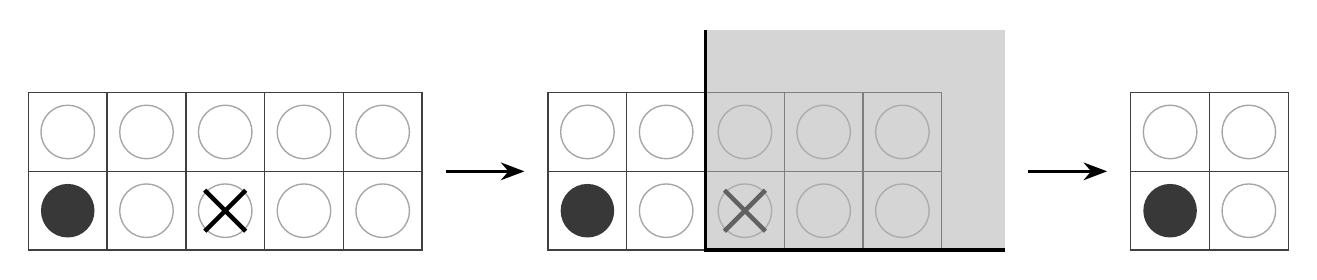
\begin{tikzpicture}[x=1mm, y=1mm]
\draw[line width=0.5pt, black!75] (0,0) rectangle ++(10,10);
\fill[black!78] (5,5) circle (3.4);
\draw[line width=0.5pt, black!75] (10,0) rectangle ++(10,10);
\draw[line width=0.5pt, black!35] (15,5) circle (3.4);
\draw[line width=0.5pt, black!75] (20,0) rectangle ++(10,10);
\draw[line width=0.5pt, black!35] (25,5) circle (3.4);
\draw[line width=0.5pt, black!75] (30,0) rectangle ++(10,10);
\draw[line width=0.5pt, black!35] (35,5) circle (3.4);
\draw[line width=0.5pt, black!75] (40,0) rectangle ++(10,10);
\draw[line width=0.5pt, black!35] (45,5) circle (3.4);
\draw[line width=0.5pt, black!75] (0,10) rectangle ++(10,10);
\draw[line width=0.5pt, black!35] (5,15) circle (3.4);
\draw[line width=0.5pt, black!75] (10,10) rectangle ++(10,10);
\draw[line width=0.5pt, black!35] (15,15) circle (3.4);
\draw[line width=0.5pt, black!75] (20,10) rectangle ++(10,10);
\draw[line width=0.5pt, black!35] (25,15) circle (3.4);
\draw[line width=0.5pt, black!75] (30,10) rectangle ++(10,10);
\draw[line width=0.5pt, black!35] (35,15) circle (3.4);
\draw[line width=0.5pt, black!75] (40,10) rectangle ++(10,10);
\draw[line width=0.5pt, black!35] (45,15) circle (3.4);
\draw[line width=1.6pt] (22.4,2.4) -- (27.6,7.6) (22.4,7.6) -- (27.6,2.4);
\draw[-{Stealth[length=3mm]}, line width=1pt] (53,10) -- ++(10,0);
\draw[line width=0.5pt, black!75] (66,0) rectangle ++(10,10);
\fill[black!78] (71,5) circle (3.4);
\draw[line width=0.5pt, black!75] (76,0) rectangle ++(10,10);
\draw[line width=0.5pt, black!35] (81,5) circle (3.4);
\draw[line width=0.5pt, black!75] (86,0) rectangle ++(10,10);
\draw[line width=0.5pt, black!35] (91,5) circle (3.4);
\draw[line width=0.5pt, black!75] (96,0) rectangle ++(10,10);
\draw[line width=0.5pt, black!35] (101,5) circle (3.4);
\draw[line width=0.5pt, black!75] (106,0) rectangle ++(10,10);
\draw[line width=0.5pt, black!35] (111,5) circle (3.4);
\draw[line width=0.5pt, black!75] (66,10) rectangle ++(10,10);
\draw[line width=0.5pt, black!35] (71,15) circle (3.4);
\draw[line width=0.5pt, black!75] (76,10) rectangle ++(10,10);
\draw[line width=0.5pt, black!35] (81,15) circle (3.4);
\draw[line width=0.5pt, black!75] (86,10) rectangle ++(10,10);
\draw[line width=0.5pt, black!35] (91,15) circle (3.4);
\draw[line width=0.5pt, black!75] (96,10) rectangle ++(10,10);
\draw[line width=0.5pt, black!35] (101,15) circle (3.4);
\draw[line width=0.5pt, black!75] (106,10) rectangle ++(10,10);
\draw[line width=0.5pt, black!35] (111,15) circle (3.4);
\draw[line width=1.6pt] (88.4,2.4) -- (93.6,7.6) (88.4,7.6) -- (93.6,2.4);
\fill[black!30, opacity=0.55] (86,0) rectangle (124,28);
\draw[line width=1.4pt] (124,0) -- (86,0) -- (86,28);
\draw[-{Stealth[length=3mm]}, line width=1pt] (127,10) -- ++(10,0);
\draw[line width=0.5pt, black!75] (140,0) rectangle ++(10,10);
\fill[black!78] (145,5) circle (3.4);
\draw[line width=0.5pt, black!75] (150,0) rectangle ++(10,10);
\draw[line width=0.5pt, black!35] (155,5) circle (3.4);
\draw[line width=0.5pt, black!75] (140,10) rectangle ++(10,10);
\draw[line width=0.5pt, black!35] (145,15) circle (3.4);
\draw[line width=0.5pt, black!75] (150,10) rectangle ++(10,10);
\draw[line width=0.5pt, black!35] (155,15) circle (3.4);
\end{tikzpicture}\par}\vspace{8mm}
\prob{1}It is your turn on each board. Mark your first bite with an X if you can make sure you win, or circle the board if you can't.\par\vspace{5mm}
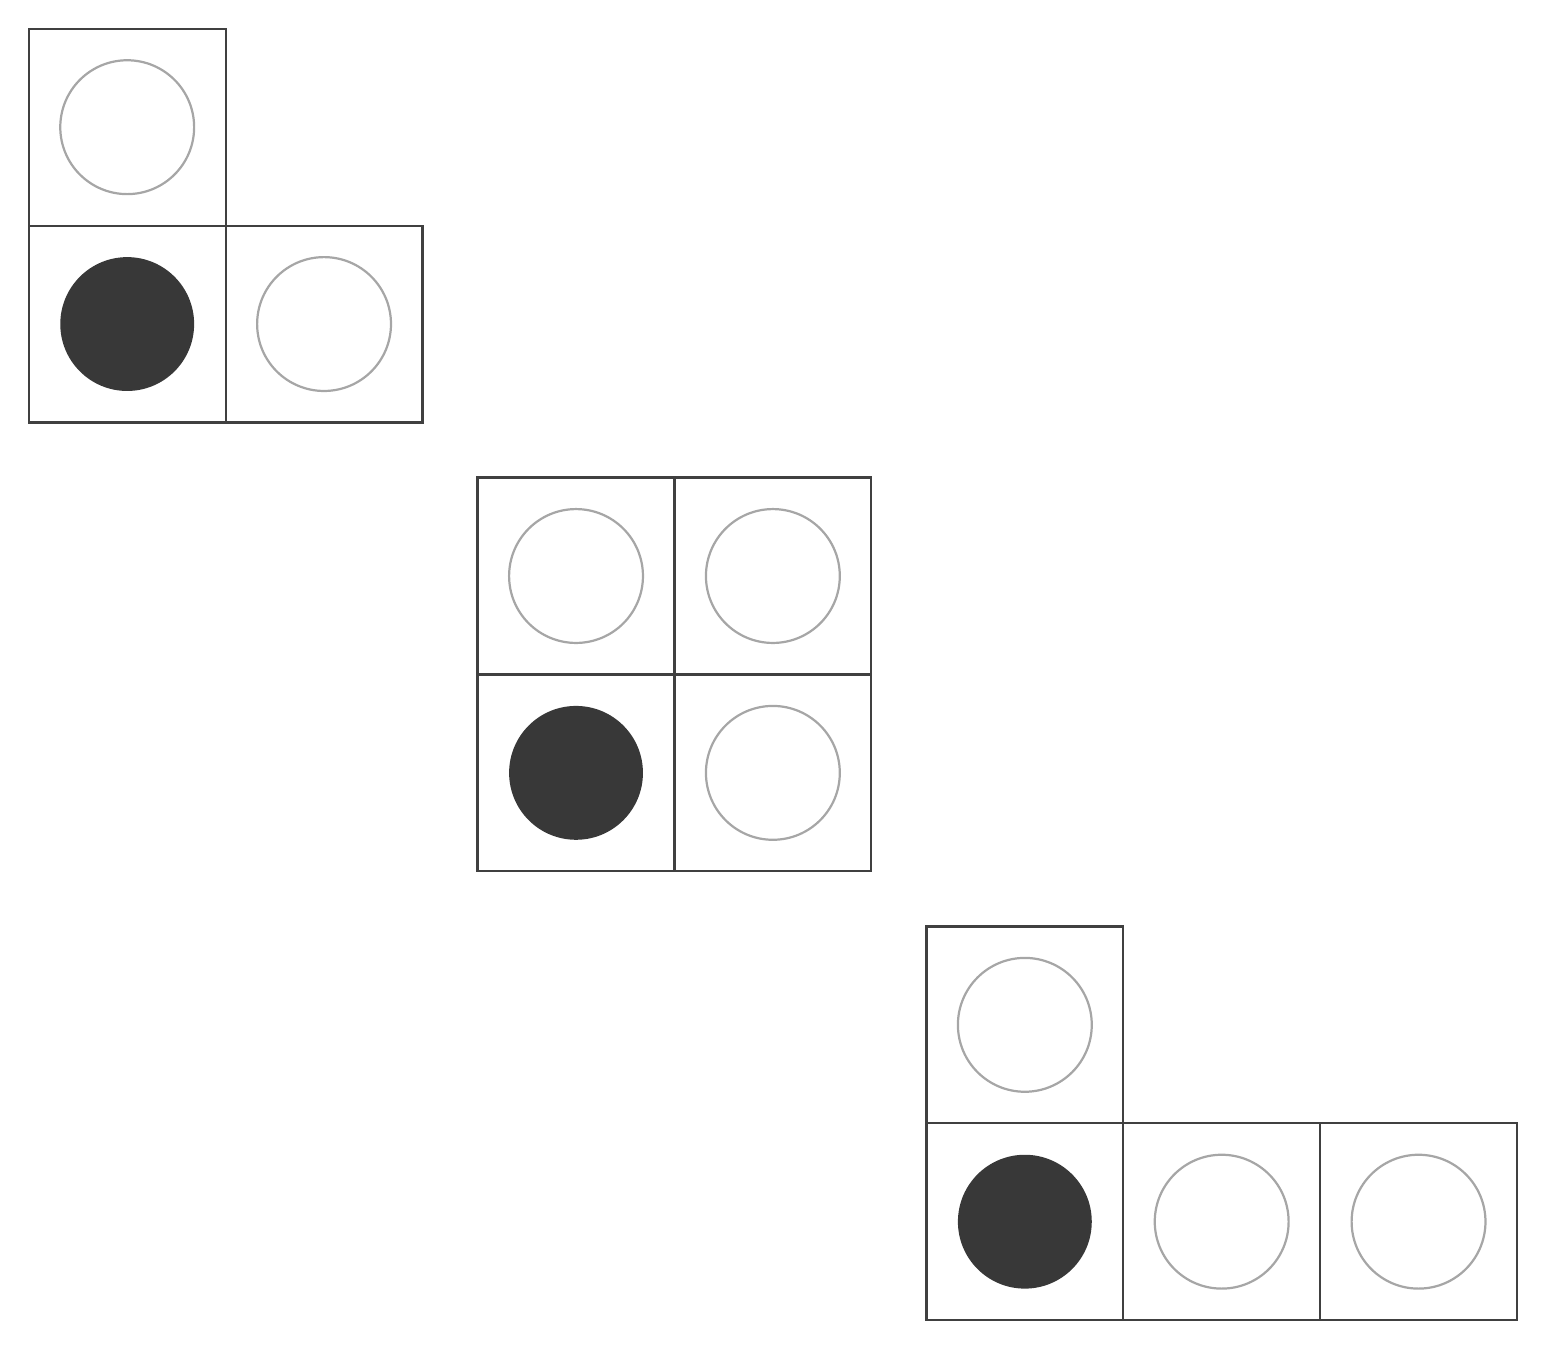
\begin{tikzpicture}[x=1mm, y=1mm]
\draw[line width=0.8pt, black!75] (0,114) rectangle ++(25,25);
\fill[black!78] (12.5,126.5) circle (8.5);
\draw[line width=0.8pt, black!75] (25,114) rectangle ++(25,25);
\draw[line width=0.8pt, black!35] (37.5,126.5) circle (8.5);
\draw[line width=0.8pt, black!75] (0,139) rectangle ++(25,25);
\draw[line width=0.8pt, black!35] (12.5,151.5) circle (8.5);
\draw[line width=0.8pt, black!75] (57,57) rectangle ++(25,25);
\fill[black!78] (69.5,69.5) circle (8.5);
\draw[line width=0.8pt, black!75] (82,57) rectangle ++(25,25);
\draw[line width=0.8pt, black!35] (94.5,69.5) circle (8.5);
\draw[line width=0.8pt, black!75] (57,82) rectangle ++(25,25);
\draw[line width=0.8pt, black!35] (69.5,94.5) circle (8.5);
\draw[line width=0.8pt, black!75] (82,82) rectangle ++(25,25);
\draw[line width=0.8pt, black!35] (94.5,94.5) circle (8.5);
\draw[line width=0.8pt, black!75] (114,0) rectangle ++(25,25);
\fill[black!78] (126.5,12.5) circle (8.5);
\draw[line width=0.8pt, black!75] (139,0) rectangle ++(25,25);
\draw[line width=0.8pt, black!35] (151.5,12.5) circle (8.5);
\draw[line width=0.8pt, black!75] (164,0) rectangle ++(25,25);
\draw[line width=0.8pt, black!35] (176.5,12.5) circle (8.5);
\draw[line width=0.8pt, black!75] (114,25) rectangle ++(25,25);
\draw[line width=0.8pt, black!35] (126.5,37.5) circle (8.5);
\end{tikzpicture}\par\vspace{0mm}
\newpage
\prob{2}Play on each board with your partner, taking turns going first. Find how to make sure you win when you go first, and mark your first bite with an X.\par\vspace{6mm}
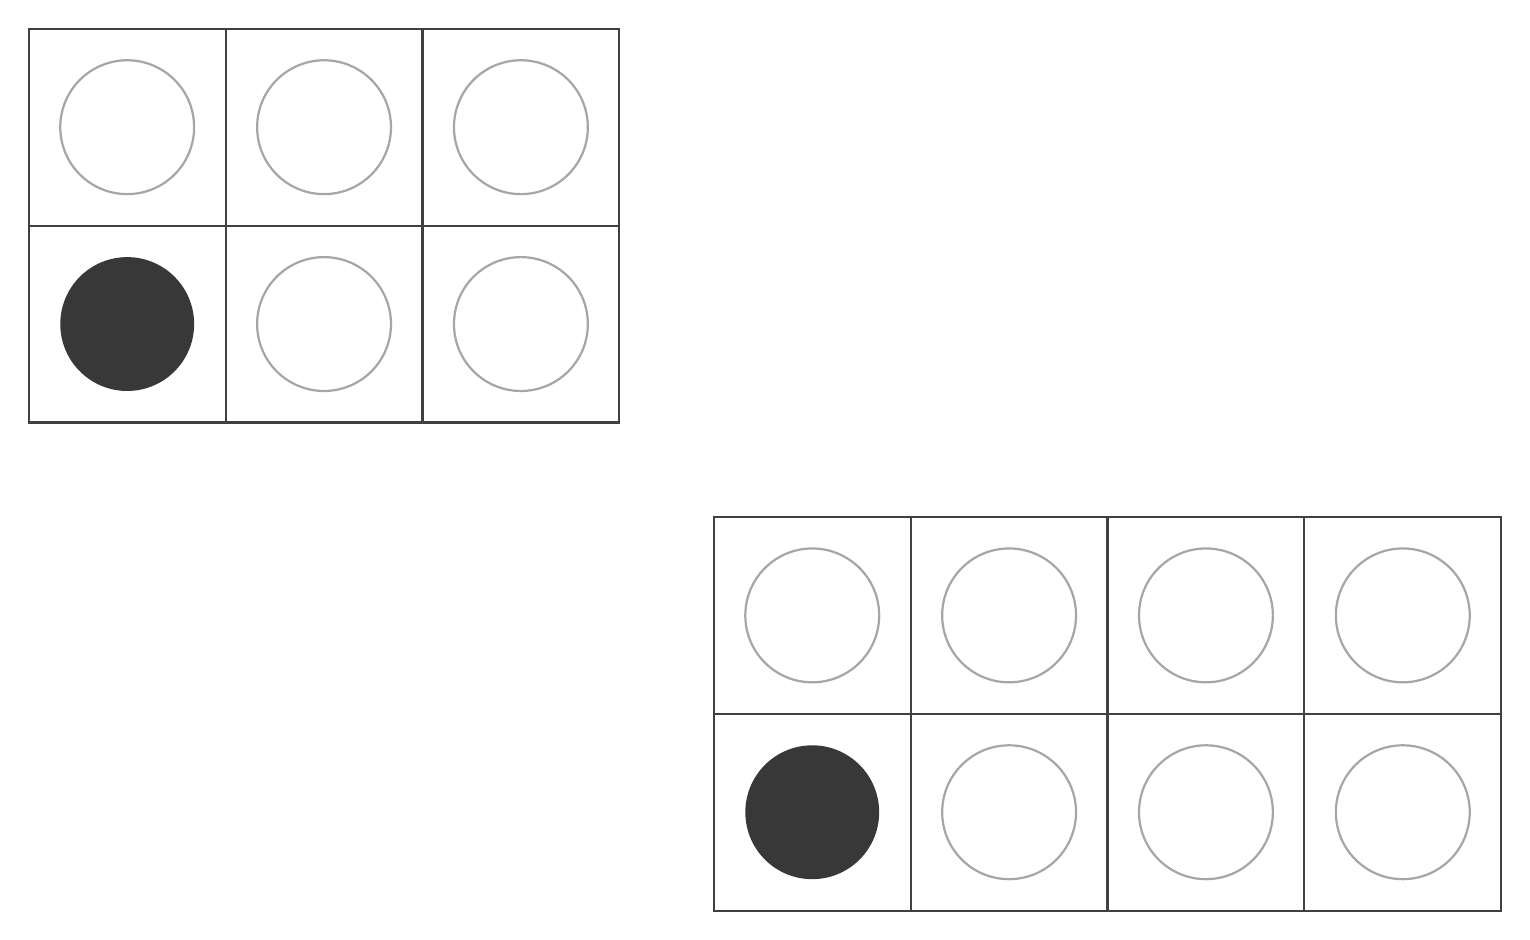
\begin{tikzpicture}[x=1mm, y=1mm]
\draw[line width=0.8pt, black!75] (0,62) rectangle ++(25,25);
\fill[black!78] (12.5,74.5) circle (8.5);
\draw[line width=0.8pt, black!75] (25,62) rectangle ++(25,25);
\draw[line width=0.8pt, black!35] (37.5,74.5) circle (8.5);
\draw[line width=0.8pt, black!75] (50,62) rectangle ++(25,25);
\draw[line width=0.8pt, black!35] (62.5,74.5) circle (8.5);
\draw[line width=0.8pt, black!75] (0,87) rectangle ++(25,25);
\draw[line width=0.8pt, black!35] (12.5,99.5) circle (8.5);
\draw[line width=0.8pt, black!75] (25,87) rectangle ++(25,25);
\draw[line width=0.8pt, black!35] (37.5,99.5) circle (8.5);
\draw[line width=0.8pt, black!75] (50,87) rectangle ++(25,25);
\draw[line width=0.8pt, black!35] (62.5,99.5) circle (8.5);
\draw[line width=0.8pt, black!75] (87,0) rectangle ++(25,25);
\fill[black!78] (99.5,12.5) circle (8.5);
\draw[line width=0.8pt, black!75] (112,0) rectangle ++(25,25);
\draw[line width=0.8pt, black!35] (124.5,12.5) circle (8.5);
\draw[line width=0.8pt, black!75] (137,0) rectangle ++(25,25);
\draw[line width=0.8pt, black!35] (149.5,12.5) circle (8.5);
\draw[line width=0.8pt, black!75] (162,0) rectangle ++(25,25);
\draw[line width=0.8pt, black!35] (174.5,12.5) circle (8.5);
\draw[line width=0.8pt, black!75] (87,25) rectangle ++(25,25);
\draw[line width=0.8pt, black!35] (99.5,37.5) circle (8.5);
\draw[line width=0.8pt, black!75] (112,25) rectangle ++(25,25);
\draw[line width=0.8pt, black!35] (124.5,37.5) circle (8.5);
\draw[line width=0.8pt, black!75] (137,25) rectangle ++(25,25);
\draw[line width=0.8pt, black!35] (149.5,37.5) circle (8.5);
\draw[line width=0.8pt, black!75] (162,25) rectangle ++(25,25);
\draw[line width=0.8pt, black!35] (174.5,37.5) circle (8.5);
\end{tikzpicture}\par\vspace{0mm}
\newpage
\prob{3}Play on each board with your partner. Circle each board where the player who goes second can make sure to win.\par\vspace{6mm}
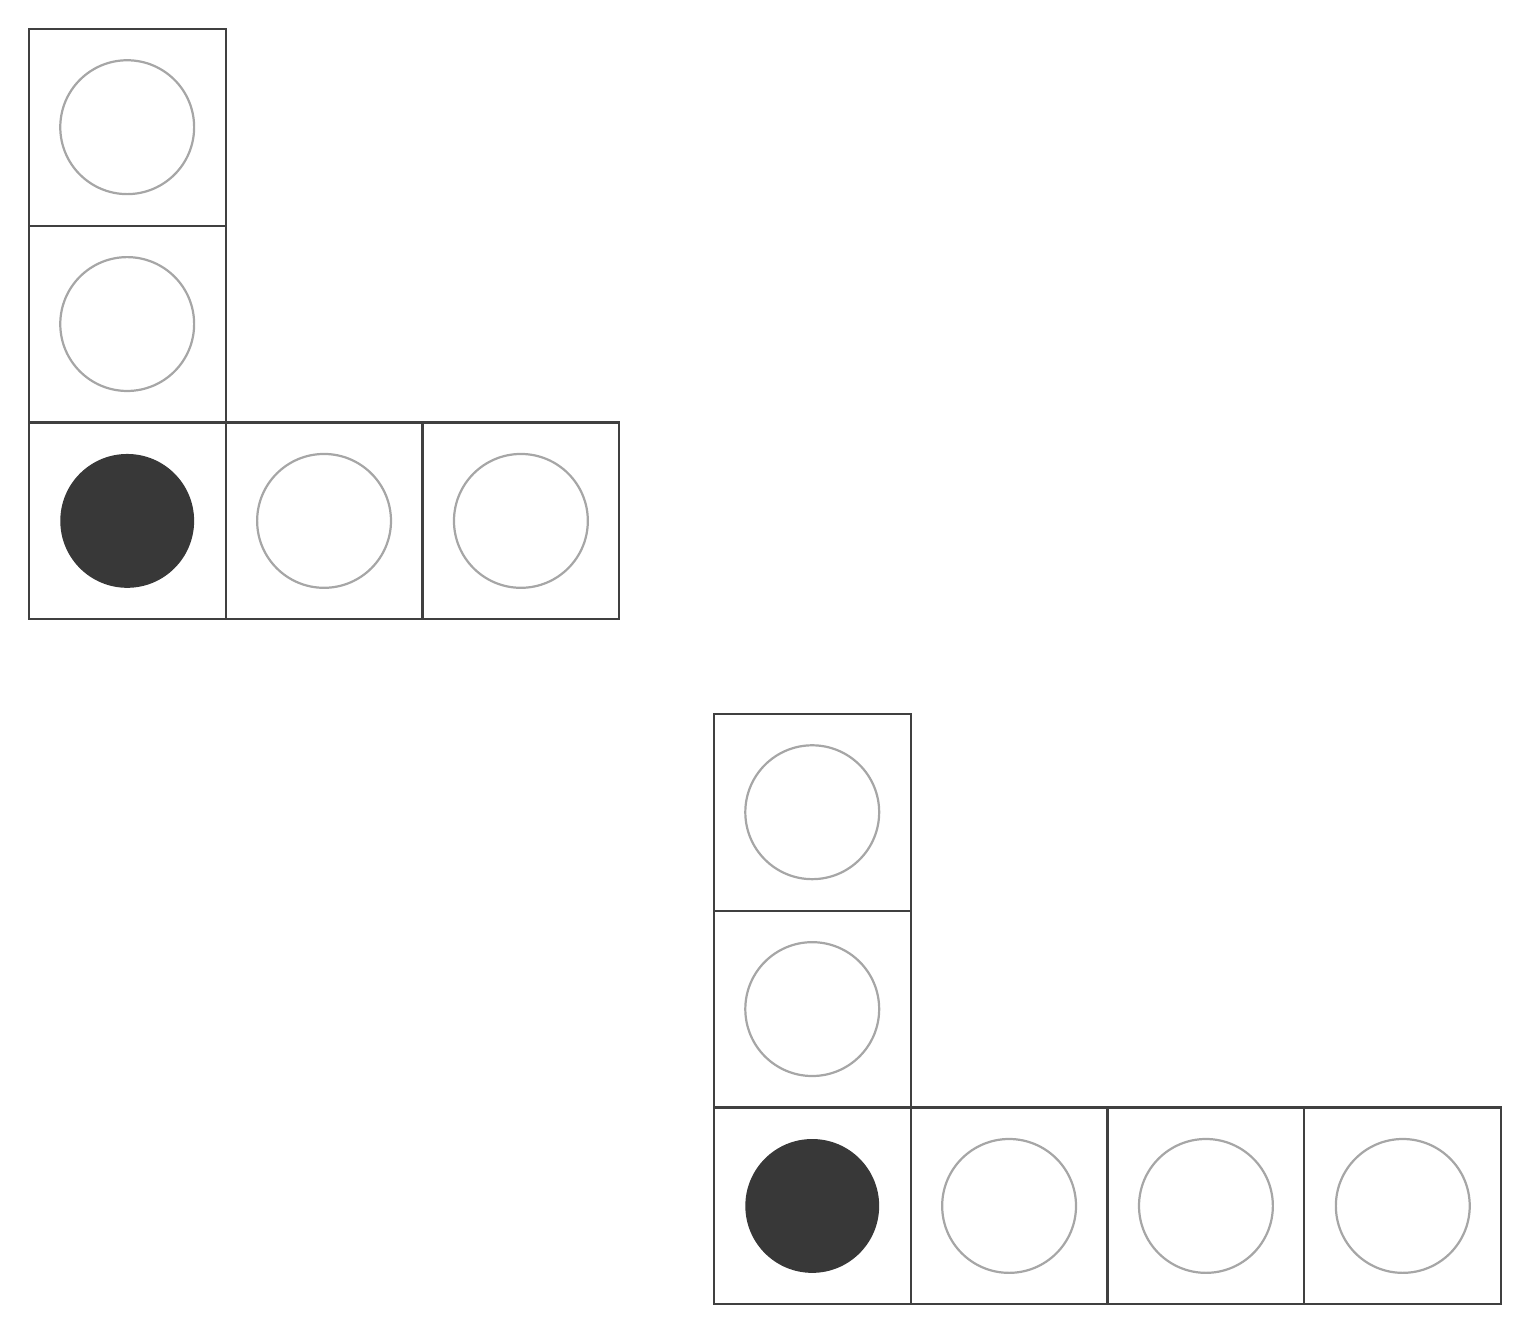
\begin{tikzpicture}[x=1mm, y=1mm]
\draw[line width=0.8pt, black!75] (0,87) rectangle ++(25,25);
\fill[black!78] (12.5,99.5) circle (8.5);
\draw[line width=0.8pt, black!75] (25,87) rectangle ++(25,25);
\draw[line width=0.8pt, black!35] (37.5,99.5) circle (8.5);
\draw[line width=0.8pt, black!75] (50,87) rectangle ++(25,25);
\draw[line width=0.8pt, black!35] (62.5,99.5) circle (8.5);
\draw[line width=0.8pt, black!75] (0,112) rectangle ++(25,25);
\draw[line width=0.8pt, black!35] (12.5,124.5) circle (8.5);
\draw[line width=0.8pt, black!75] (0,137) rectangle ++(25,25);
\draw[line width=0.8pt, black!35] (12.5,149.5) circle (8.5);
\draw[line width=0.8pt, black!75] (87,0) rectangle ++(25,25);
\fill[black!78] (99.5,12.5) circle (8.5);
\draw[line width=0.8pt, black!75] (112,0) rectangle ++(25,25);
\draw[line width=0.8pt, black!35] (124.5,12.5) circle (8.5);
\draw[line width=0.8pt, black!75] (137,0) rectangle ++(25,25);
\draw[line width=0.8pt, black!35] (149.5,12.5) circle (8.5);
\draw[line width=0.8pt, black!75] (162,0) rectangle ++(25,25);
\draw[line width=0.8pt, black!35] (174.5,12.5) circle (8.5);
\draw[line width=0.8pt, black!75] (87,25) rectangle ++(25,25);
\draw[line width=0.8pt, black!35] (99.5,37.5) circle (8.5);
\draw[line width=0.8pt, black!75] (87,50) rectangle ++(25,25);
\draw[line width=0.8pt, black!35] (99.5,62.5) circle (8.5);
\end{tikzpicture}\par\vspace{0mm}
\newpage
\prob{4}Play on each board with your partner, taking turns going first. Find how to make sure you win when you go first, and mark your first bite with an X.\par\vspace{6mm}
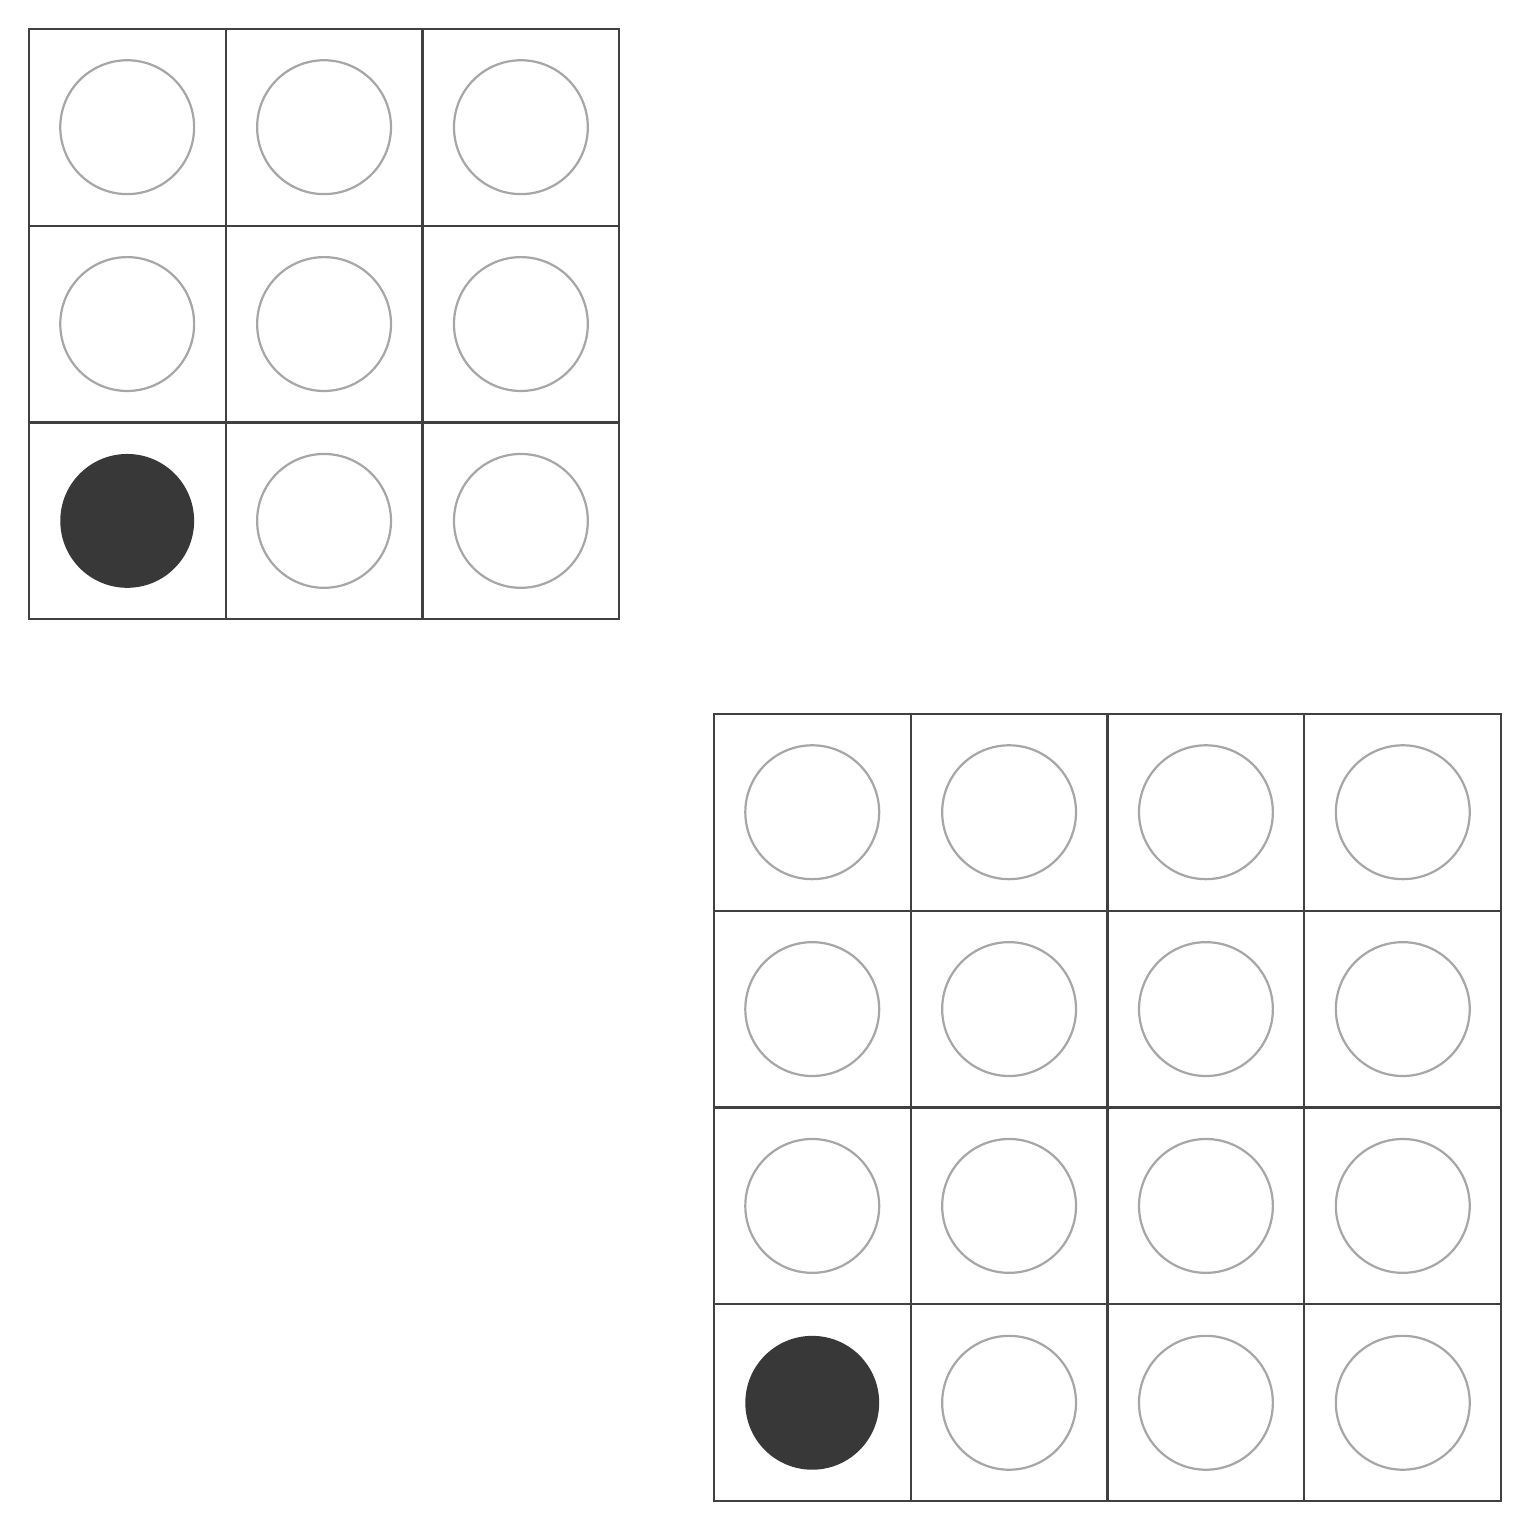
\begin{tikzpicture}[x=1mm, y=1mm]
\draw[line width=0.8pt, black!75] (0,112) rectangle ++(25,25);
\fill[black!78] (12.5,124.5) circle (8.5);
\draw[line width=0.8pt, black!75] (25,112) rectangle ++(25,25);
\draw[line width=0.8pt, black!35] (37.5,124.5) circle (8.5);
\draw[line width=0.8pt, black!75] (50,112) rectangle ++(25,25);
\draw[line width=0.8pt, black!35] (62.5,124.5) circle (8.5);
\draw[line width=0.8pt, black!75] (0,137) rectangle ++(25,25);
\draw[line width=0.8pt, black!35] (12.5,149.5) circle (8.5);
\draw[line width=0.8pt, black!75] (25,137) rectangle ++(25,25);
\draw[line width=0.8pt, black!35] (37.5,149.5) circle (8.5);
\draw[line width=0.8pt, black!75] (50,137) rectangle ++(25,25);
\draw[line width=0.8pt, black!35] (62.5,149.5) circle (8.5);
\draw[line width=0.8pt, black!75] (0,162) rectangle ++(25,25);
\draw[line width=0.8pt, black!35] (12.5,174.5) circle (8.5);
\draw[line width=0.8pt, black!75] (25,162) rectangle ++(25,25);
\draw[line width=0.8pt, black!35] (37.5,174.5) circle (8.5);
\draw[line width=0.8pt, black!75] (50,162) rectangle ++(25,25);
\draw[line width=0.8pt, black!35] (62.5,174.5) circle (8.5);
\draw[line width=0.8pt, black!75] (87,0) rectangle ++(25,25);
\fill[black!78] (99.5,12.5) circle (8.5);
\draw[line width=0.8pt, black!75] (112,0) rectangle ++(25,25);
\draw[line width=0.8pt, black!35] (124.5,12.5) circle (8.5);
\draw[line width=0.8pt, black!75] (137,0) rectangle ++(25,25);
\draw[line width=0.8pt, black!35] (149.5,12.5) circle (8.5);
\draw[line width=0.8pt, black!75] (162,0) rectangle ++(25,25);
\draw[line width=0.8pt, black!35] (174.5,12.5) circle (8.5);
\draw[line width=0.8pt, black!75] (87,25) rectangle ++(25,25);
\draw[line width=0.8pt, black!35] (99.5,37.5) circle (8.5);
\draw[line width=0.8pt, black!75] (112,25) rectangle ++(25,25);
\draw[line width=0.8pt, black!35] (124.5,37.5) circle (8.5);
\draw[line width=0.8pt, black!75] (137,25) rectangle ++(25,25);
\draw[line width=0.8pt, black!35] (149.5,37.5) circle (8.5);
\draw[line width=0.8pt, black!75] (162,25) rectangle ++(25,25);
\draw[line width=0.8pt, black!35] (174.5,37.5) circle (8.5);
\draw[line width=0.8pt, black!75] (87,50) rectangle ++(25,25);
\draw[line width=0.8pt, black!35] (99.5,62.5) circle (8.5);
\draw[line width=0.8pt, black!75] (112,50) rectangle ++(25,25);
\draw[line width=0.8pt, black!35] (124.5,62.5) circle (8.5);
\draw[line width=0.8pt, black!75] (137,50) rectangle ++(25,25);
\draw[line width=0.8pt, black!35] (149.5,62.5) circle (8.5);
\draw[line width=0.8pt, black!75] (162,50) rectangle ++(25,25);
\draw[line width=0.8pt, black!35] (174.5,62.5) circle (8.5);
\draw[line width=0.8pt, black!75] (87,75) rectangle ++(25,25);
\draw[line width=0.8pt, black!35] (99.5,87.5) circle (8.5);
\draw[line width=0.8pt, black!75] (112,75) rectangle ++(25,25);
\draw[line width=0.8pt, black!35] (124.5,87.5) circle (8.5);
\draw[line width=0.8pt, black!75] (137,75) rectangle ++(25,25);
\draw[line width=0.8pt, black!35] (149.5,87.5) circle (8.5);
\draw[line width=0.8pt, black!75] (162,75) rectangle ++(25,25);
\draw[line width=0.8pt, black!35] (174.5,87.5) circle (8.5);
\end{tikzpicture}\par\vspace{0mm}
\newpage
\prob{5}Play on this board with your partner, taking turns going first. Find how to make sure you win when you go first, and mark your first bite with an X.\par\vspace{6mm}
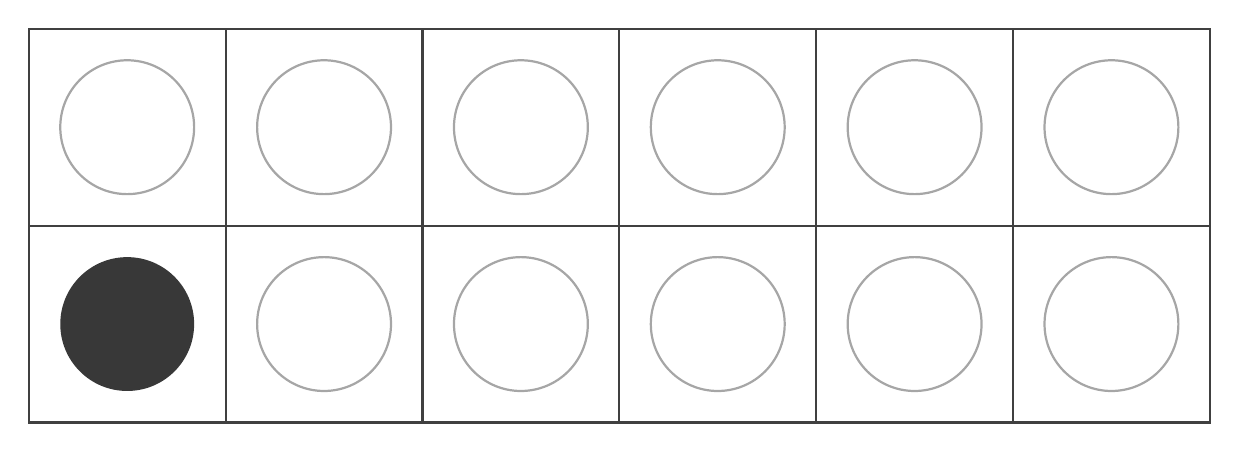
\begin{tikzpicture}[x=1mm, y=1mm]
\draw[line width=0.8pt, black!75] (0,0) rectangle ++(25,25);
\fill[black!78] (12.5,12.5) circle (8.5);
\draw[line width=0.8pt, black!75] (25,0) rectangle ++(25,25);
\draw[line width=0.8pt, black!35] (37.5,12.5) circle (8.5);
\draw[line width=0.8pt, black!75] (50,0) rectangle ++(25,25);
\draw[line width=0.8pt, black!35] (62.5,12.5) circle (8.5);
\draw[line width=0.8pt, black!75] (75,0) rectangle ++(25,25);
\draw[line width=0.8pt, black!35] (87.5,12.5) circle (8.5);
\draw[line width=0.8pt, black!75] (100,0) rectangle ++(25,25);
\draw[line width=0.8pt, black!35] (112.5,12.5) circle (8.5);
\draw[line width=0.8pt, black!75] (125,0) rectangle ++(25,25);
\draw[line width=0.8pt, black!35] (137.5,12.5) circle (8.5);
\draw[line width=0.8pt, black!75] (0,25) rectangle ++(25,25);
\draw[line width=0.8pt, black!35] (12.5,37.5) circle (8.5);
\draw[line width=0.8pt, black!75] (25,25) rectangle ++(25,25);
\draw[line width=0.8pt, black!35] (37.5,37.5) circle (8.5);
\draw[line width=0.8pt, black!75] (50,25) rectangle ++(25,25);
\draw[line width=0.8pt, black!35] (62.5,37.5) circle (8.5);
\draw[line width=0.8pt, black!75] (75,25) rectangle ++(25,25);
\draw[line width=0.8pt, black!35] (87.5,37.5) circle (8.5);
\draw[line width=0.8pt, black!75] (100,25) rectangle ++(25,25);
\draw[line width=0.8pt, black!35] (112.5,37.5) circle (8.5);
\draw[line width=0.8pt, black!75] (125,25) rectangle ++(25,25);
\draw[line width=0.8pt, black!35] (137.5,37.5) circle (8.5);
\end{tikzpicture}\par\vspace{0mm}
\newpage
\prob{6}Take bites from a full 4 by 4 board to make a board where the player who goes second can make sure to win. Color each board you find on a grid.\par\vspace{8mm}
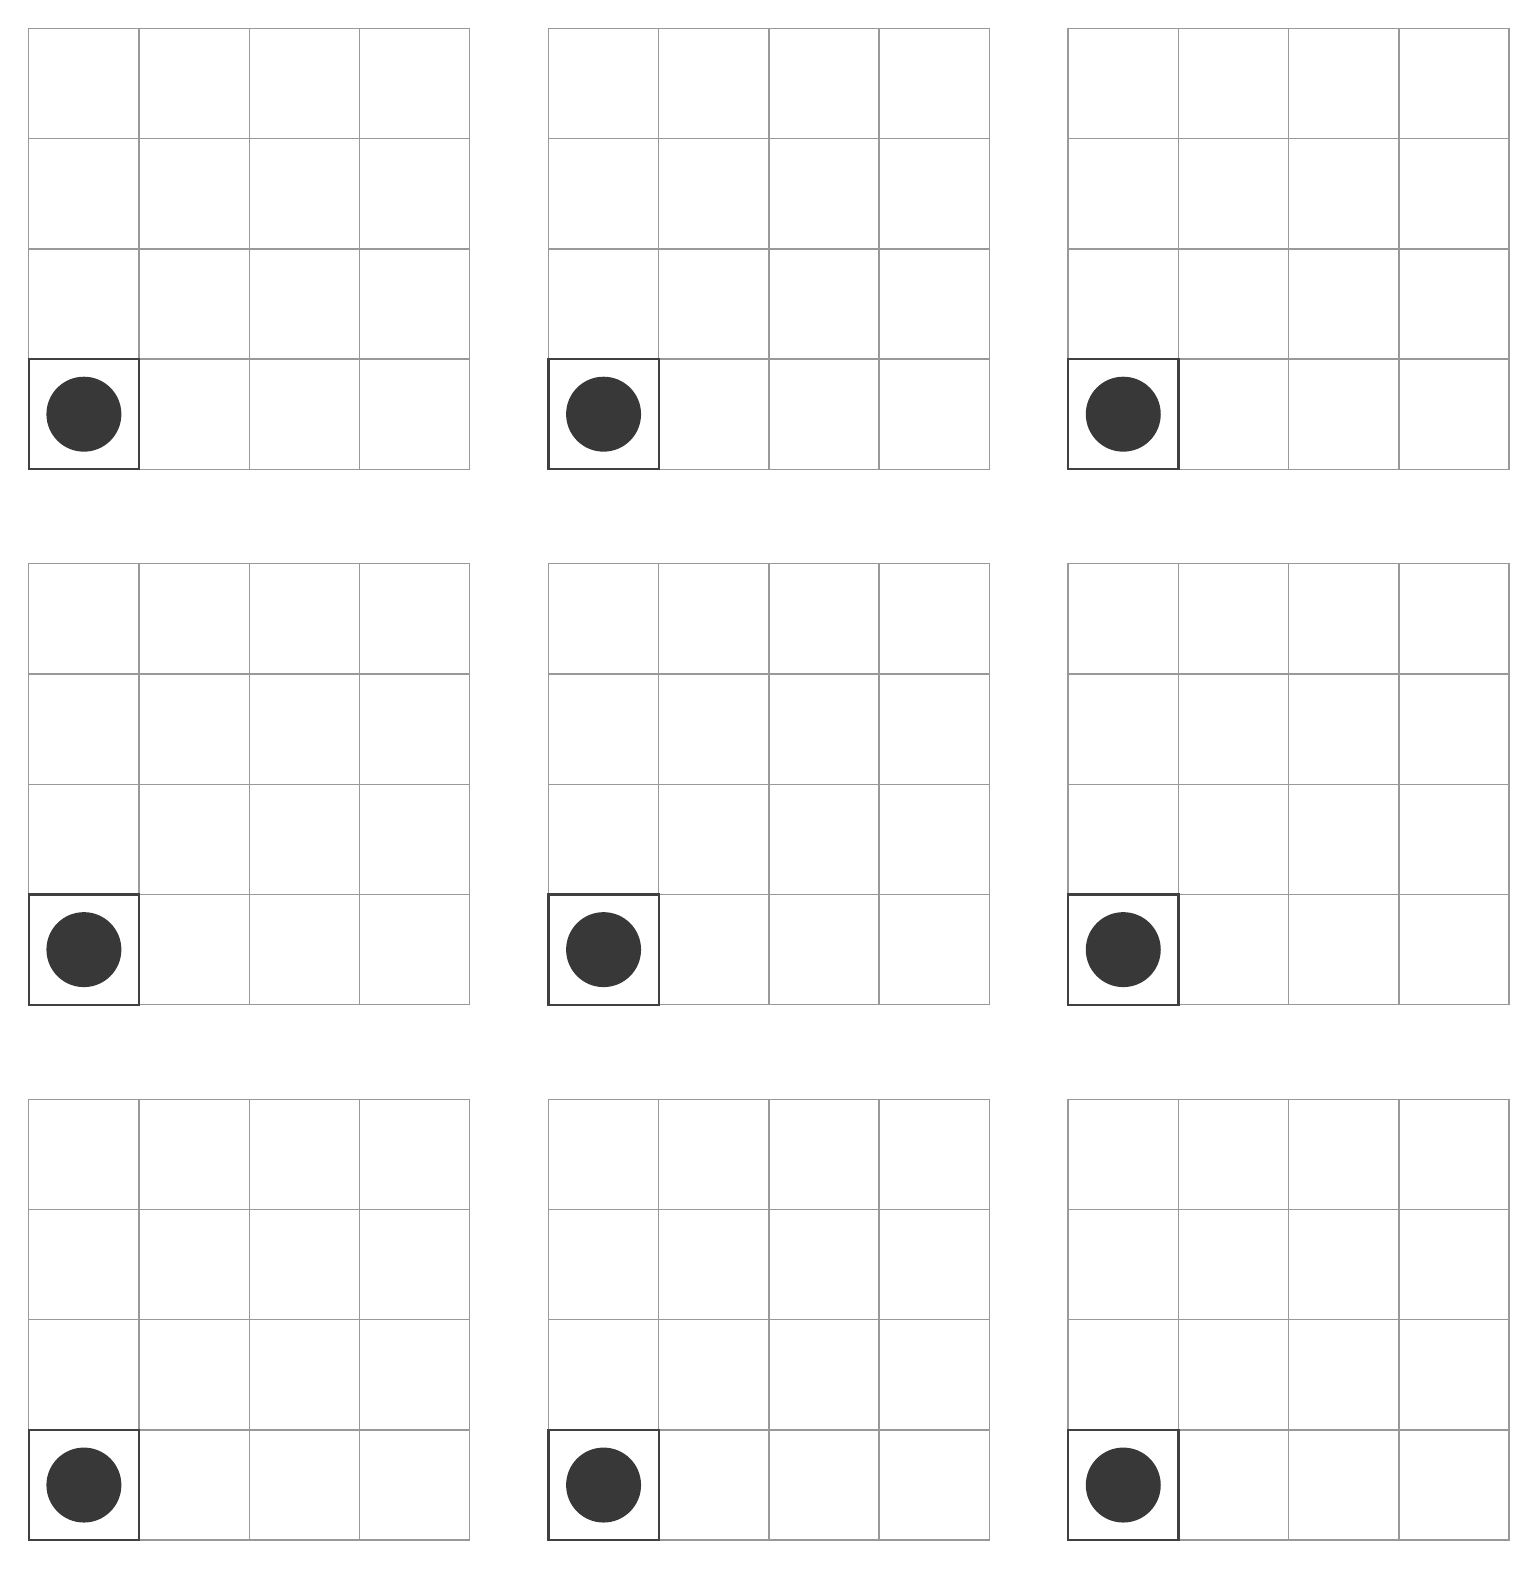
\begin{tikzpicture}[x=1mm, y=1mm]
\draw[line width=0.5pt, black!40] (0,0) rectangle ++(14,14);
\draw[line width=0.5pt, black!40] (14,0) rectangle ++(14,14);
\draw[line width=0.5pt, black!40] (28,0) rectangle ++(14,14);
\draw[line width=0.5pt, black!40] (42,0) rectangle ++(14,14);
\draw[line width=0.5pt, black!40] (0,14) rectangle ++(14,14);
\draw[line width=0.5pt, black!40] (14,14) rectangle ++(14,14);
\draw[line width=0.5pt, black!40] (28,14) rectangle ++(14,14);
\draw[line width=0.5pt, black!40] (42,14) rectangle ++(14,14);
\draw[line width=0.5pt, black!40] (0,28) rectangle ++(14,14);
\draw[line width=0.5pt, black!40] (14,28) rectangle ++(14,14);
\draw[line width=0.5pt, black!40] (28,28) rectangle ++(14,14);
\draw[line width=0.5pt, black!40] (42,28) rectangle ++(14,14);
\draw[line width=0.5pt, black!40] (0,42) rectangle ++(14,14);
\draw[line width=0.5pt, black!40] (14,42) rectangle ++(14,14);
\draw[line width=0.5pt, black!40] (28,42) rectangle ++(14,14);
\draw[line width=0.5pt, black!40] (42,42) rectangle ++(14,14);
\fill[black!78] (7,7) circle (4.76);
\draw[line width=0.8pt, black!75] (0,0) rectangle ++(14,14);
\draw[line width=0.5pt, black!40] (66,0) rectangle ++(14,14);
\draw[line width=0.5pt, black!40] (80,0) rectangle ++(14,14);
\draw[line width=0.5pt, black!40] (94,0) rectangle ++(14,14);
\draw[line width=0.5pt, black!40] (108,0) rectangle ++(14,14);
\draw[line width=0.5pt, black!40] (66,14) rectangle ++(14,14);
\draw[line width=0.5pt, black!40] (80,14) rectangle ++(14,14);
\draw[line width=0.5pt, black!40] (94,14) rectangle ++(14,14);
\draw[line width=0.5pt, black!40] (108,14) rectangle ++(14,14);
\draw[line width=0.5pt, black!40] (66,28) rectangle ++(14,14);
\draw[line width=0.5pt, black!40] (80,28) rectangle ++(14,14);
\draw[line width=0.5pt, black!40] (94,28) rectangle ++(14,14);
\draw[line width=0.5pt, black!40] (108,28) rectangle ++(14,14);
\draw[line width=0.5pt, black!40] (66,42) rectangle ++(14,14);
\draw[line width=0.5pt, black!40] (80,42) rectangle ++(14,14);
\draw[line width=0.5pt, black!40] (94,42) rectangle ++(14,14);
\draw[line width=0.5pt, black!40] (108,42) rectangle ++(14,14);
\fill[black!78] (73,7) circle (4.76);
\draw[line width=0.8pt, black!75] (66,0) rectangle ++(14,14);
\draw[line width=0.5pt, black!40] (132,0) rectangle ++(14,14);
\draw[line width=0.5pt, black!40] (146,0) rectangle ++(14,14);
\draw[line width=0.5pt, black!40] (160,0) rectangle ++(14,14);
\draw[line width=0.5pt, black!40] (174,0) rectangle ++(14,14);
\draw[line width=0.5pt, black!40] (132,14) rectangle ++(14,14);
\draw[line width=0.5pt, black!40] (146,14) rectangle ++(14,14);
\draw[line width=0.5pt, black!40] (160,14) rectangle ++(14,14);
\draw[line width=0.5pt, black!40] (174,14) rectangle ++(14,14);
\draw[line width=0.5pt, black!40] (132,28) rectangle ++(14,14);
\draw[line width=0.5pt, black!40] (146,28) rectangle ++(14,14);
\draw[line width=0.5pt, black!40] (160,28) rectangle ++(14,14);
\draw[line width=0.5pt, black!40] (174,28) rectangle ++(14,14);
\draw[line width=0.5pt, black!40] (132,42) rectangle ++(14,14);
\draw[line width=0.5pt, black!40] (146,42) rectangle ++(14,14);
\draw[line width=0.5pt, black!40] (160,42) rectangle ++(14,14);
\draw[line width=0.5pt, black!40] (174,42) rectangle ++(14,14);
\fill[black!78] (139,7) circle (4.76);
\draw[line width=0.8pt, black!75] (132,0) rectangle ++(14,14);
\draw[line width=0.5pt, black!40] (0,-68) rectangle ++(14,14);
\draw[line width=0.5pt, black!40] (14,-68) rectangle ++(14,14);
\draw[line width=0.5pt, black!40] (28,-68) rectangle ++(14,14);
\draw[line width=0.5pt, black!40] (42,-68) rectangle ++(14,14);
\draw[line width=0.5pt, black!40] (0,-54) rectangle ++(14,14);
\draw[line width=0.5pt, black!40] (14,-54) rectangle ++(14,14);
\draw[line width=0.5pt, black!40] (28,-54) rectangle ++(14,14);
\draw[line width=0.5pt, black!40] (42,-54) rectangle ++(14,14);
\draw[line width=0.5pt, black!40] (0,-40) rectangle ++(14,14);
\draw[line width=0.5pt, black!40] (14,-40) rectangle ++(14,14);
\draw[line width=0.5pt, black!40] (28,-40) rectangle ++(14,14);
\draw[line width=0.5pt, black!40] (42,-40) rectangle ++(14,14);
\draw[line width=0.5pt, black!40] (0,-26) rectangle ++(14,14);
\draw[line width=0.5pt, black!40] (14,-26) rectangle ++(14,14);
\draw[line width=0.5pt, black!40] (28,-26) rectangle ++(14,14);
\draw[line width=0.5pt, black!40] (42,-26) rectangle ++(14,14);
\fill[black!78] (7,-61) circle (4.76);
\draw[line width=0.8pt, black!75] (0,-68) rectangle ++(14,14);
\draw[line width=0.5pt, black!40] (66,-68) rectangle ++(14,14);
\draw[line width=0.5pt, black!40] (80,-68) rectangle ++(14,14);
\draw[line width=0.5pt, black!40] (94,-68) rectangle ++(14,14);
\draw[line width=0.5pt, black!40] (108,-68) rectangle ++(14,14);
\draw[line width=0.5pt, black!40] (66,-54) rectangle ++(14,14);
\draw[line width=0.5pt, black!40] (80,-54) rectangle ++(14,14);
\draw[line width=0.5pt, black!40] (94,-54) rectangle ++(14,14);
\draw[line width=0.5pt, black!40] (108,-54) rectangle ++(14,14);
\draw[line width=0.5pt, black!40] (66,-40) rectangle ++(14,14);
\draw[line width=0.5pt, black!40] (80,-40) rectangle ++(14,14);
\draw[line width=0.5pt, black!40] (94,-40) rectangle ++(14,14);
\draw[line width=0.5pt, black!40] (108,-40) rectangle ++(14,14);
\draw[line width=0.5pt, black!40] (66,-26) rectangle ++(14,14);
\draw[line width=0.5pt, black!40] (80,-26) rectangle ++(14,14);
\draw[line width=0.5pt, black!40] (94,-26) rectangle ++(14,14);
\draw[line width=0.5pt, black!40] (108,-26) rectangle ++(14,14);
\fill[black!78] (73,-61) circle (4.76);
\draw[line width=0.8pt, black!75] (66,-68) rectangle ++(14,14);
\draw[line width=0.5pt, black!40] (132,-68) rectangle ++(14,14);
\draw[line width=0.5pt, black!40] (146,-68) rectangle ++(14,14);
\draw[line width=0.5pt, black!40] (160,-68) rectangle ++(14,14);
\draw[line width=0.5pt, black!40] (174,-68) rectangle ++(14,14);
\draw[line width=0.5pt, black!40] (132,-54) rectangle ++(14,14);
\draw[line width=0.5pt, black!40] (146,-54) rectangle ++(14,14);
\draw[line width=0.5pt, black!40] (160,-54) rectangle ++(14,14);
\draw[line width=0.5pt, black!40] (174,-54) rectangle ++(14,14);
\draw[line width=0.5pt, black!40] (132,-40) rectangle ++(14,14);
\draw[line width=0.5pt, black!40] (146,-40) rectangle ++(14,14);
\draw[line width=0.5pt, black!40] (160,-40) rectangle ++(14,14);
\draw[line width=0.5pt, black!40] (174,-40) rectangle ++(14,14);
\draw[line width=0.5pt, black!40] (132,-26) rectangle ++(14,14);
\draw[line width=0.5pt, black!40] (146,-26) rectangle ++(14,14);
\draw[line width=0.5pt, black!40] (160,-26) rectangle ++(14,14);
\draw[line width=0.5pt, black!40] (174,-26) rectangle ++(14,14);
\fill[black!78] (139,-61) circle (4.76);
\draw[line width=0.8pt, black!75] (132,-68) rectangle ++(14,14);
\draw[line width=0.5pt, black!40] (0,-136) rectangle ++(14,14);
\draw[line width=0.5pt, black!40] (14,-136) rectangle ++(14,14);
\draw[line width=0.5pt, black!40] (28,-136) rectangle ++(14,14);
\draw[line width=0.5pt, black!40] (42,-136) rectangle ++(14,14);
\draw[line width=0.5pt, black!40] (0,-122) rectangle ++(14,14);
\draw[line width=0.5pt, black!40] (14,-122) rectangle ++(14,14);
\draw[line width=0.5pt, black!40] (28,-122) rectangle ++(14,14);
\draw[line width=0.5pt, black!40] (42,-122) rectangle ++(14,14);
\draw[line width=0.5pt, black!40] (0,-108) rectangle ++(14,14);
\draw[line width=0.5pt, black!40] (14,-108) rectangle ++(14,14);
\draw[line width=0.5pt, black!40] (28,-108) rectangle ++(14,14);
\draw[line width=0.5pt, black!40] (42,-108) rectangle ++(14,14);
\draw[line width=0.5pt, black!40] (0,-94) rectangle ++(14,14);
\draw[line width=0.5pt, black!40] (14,-94) rectangle ++(14,14);
\draw[line width=0.5pt, black!40] (28,-94) rectangle ++(14,14);
\draw[line width=0.5pt, black!40] (42,-94) rectangle ++(14,14);
\fill[black!78] (7,-129) circle (4.76);
\draw[line width=0.8pt, black!75] (0,-136) rectangle ++(14,14);
\draw[line width=0.5pt, black!40] (66,-136) rectangle ++(14,14);
\draw[line width=0.5pt, black!40] (80,-136) rectangle ++(14,14);
\draw[line width=0.5pt, black!40] (94,-136) rectangle ++(14,14);
\draw[line width=0.5pt, black!40] (108,-136) rectangle ++(14,14);
\draw[line width=0.5pt, black!40] (66,-122) rectangle ++(14,14);
\draw[line width=0.5pt, black!40] (80,-122) rectangle ++(14,14);
\draw[line width=0.5pt, black!40] (94,-122) rectangle ++(14,14);
\draw[line width=0.5pt, black!40] (108,-122) rectangle ++(14,14);
\draw[line width=0.5pt, black!40] (66,-108) rectangle ++(14,14);
\draw[line width=0.5pt, black!40] (80,-108) rectangle ++(14,14);
\draw[line width=0.5pt, black!40] (94,-108) rectangle ++(14,14);
\draw[line width=0.5pt, black!40] (108,-108) rectangle ++(14,14);
\draw[line width=0.5pt, black!40] (66,-94) rectangle ++(14,14);
\draw[line width=0.5pt, black!40] (80,-94) rectangle ++(14,14);
\draw[line width=0.5pt, black!40] (94,-94) rectangle ++(14,14);
\draw[line width=0.5pt, black!40] (108,-94) rectangle ++(14,14);
\fill[black!78] (73,-129) circle (4.76);
\draw[line width=0.8pt, black!75] (66,-136) rectangle ++(14,14);
\draw[line width=0.5pt, black!40] (132,-136) rectangle ++(14,14);
\draw[line width=0.5pt, black!40] (146,-136) rectangle ++(14,14);
\draw[line width=0.5pt, black!40] (160,-136) rectangle ++(14,14);
\draw[line width=0.5pt, black!40] (174,-136) rectangle ++(14,14);
\draw[line width=0.5pt, black!40] (132,-122) rectangle ++(14,14);
\draw[line width=0.5pt, black!40] (146,-122) rectangle ++(14,14);
\draw[line width=0.5pt, black!40] (160,-122) rectangle ++(14,14);
\draw[line width=0.5pt, black!40] (174,-122) rectangle ++(14,14);
\draw[line width=0.5pt, black!40] (132,-108) rectangle ++(14,14);
\draw[line width=0.5pt, black!40] (146,-108) rectangle ++(14,14);
\draw[line width=0.5pt, black!40] (160,-108) rectangle ++(14,14);
\draw[line width=0.5pt, black!40] (174,-108) rectangle ++(14,14);
\draw[line width=0.5pt, black!40] (132,-94) rectangle ++(14,14);
\draw[line width=0.5pt, black!40] (146,-94) rectangle ++(14,14);
\draw[line width=0.5pt, black!40] (160,-94) rectangle ++(14,14);
\draw[line width=0.5pt, black!40] (174,-94) rectangle ++(14,14);
\fill[black!78] (139,-129) circle (4.76);
\draw[line width=0.8pt, black!75] (132,-136) rectangle ++(14,14);
\end{tikzpicture}\par\vspace{0mm}

\end{document}
